\section{Experiments}
\label{sec:experiment}

This section reports the five comparison families that the matrix of Section~\ref{sec:our_work} supports.

\subsection{Protocol}
\label{sec:exp-protocol}

All runs share an identical training harness. Gradient accumulation reaches an effective batch size of 128; gradients are $\ell_2$-clipped at 9 for BiLSTM runs and left unclipped for Muon-trained Transformer runs \citep{jordan2024muon}. The pretrained embedding table is frozen. Reported numbers are dev UAS and dev LAS, computed by the standard evaluator with punctuation filtered out. Each configuration is a single seed; within-seed variance on this corpus is below $0.2$ UAS for the few runs we re-executed.

\paragraph{Hardware and released artifacts.} All compute-heavy training runs were executed on server 4, an A800 machine with eight 80GB GPUs, CUDA 12.9, 1TB RAM, and an 85TB shared data volume mounted at \texttt{/essfs100}. The code repository is released at \url{https://github.com/kyksj-1/Dependency-Parsing-LXQ}; the full \texttt{Output/} directory, including checkpoints, logs, plots and run summaries, is released separately at \url{https://huggingface.co/kyksj/Dependency-Parsing} to keep large binary artifacts out of GitHub.

\subsection{A. Word vector dimensionality}
\label{sec:exp-dim}

We compare the 300-dimensional mixed-large embedding against a 100-dimensional version obtained by post-hoc PCA on the same corpus (retains $73.5\%$ variance). The two runs differ only in this single field. Results: $86.43$ UAS at 300d, $86.14$ UAS at 100d. A $0.29$-point drop for discarding two thirds of the encoded variance indicates that most of the parsing-relevant signal lies in the top principal directions of the embedding.

\subsection{B. Word vector domain}
\label{sec:exp-domain}

Fixing dimensionality at 300, we vary the source corpus across mixed-large, Renmin Ribao (newspaper), Zhihu (Q\&A), and a literature-only release. UAS spans $86.23$--$86.43$, a $0.20$-point range. Domain choice has near-zero effect at this scale; the meaningful gap is between any pretrained vector and from-scratch ($84.84$).

\subsection{C. Optimizer (BiLSTM encoder)}
\label{sec:exp-optimizer}

Holding the encoder at BiLSTM and the word vectors at mixed-large 300d:
\begin{itemize}[leftmargin=*, itemsep=2pt]
  \item Adam, 50 epochs: $86.43$ UAS (baseline).
  \item SGD, 50 epochs, $\eta{=}10^{-2}$, no momentum: $17.66$ UAS. Negative control confirming that adaptive optimization is required.
  \item Muon, 50 epochs: $85.51$ UAS, $0.92$ below Adam.
  \item Muon, 100 epochs with warmup--cosine: $\mathbf{86.93}$ UAS, $+0.50$ over Adam.
\end{itemize}
Muon overtakes Adam only when the schedule is extended to 100 epochs with warmup; at 50 epochs the orthogonalized updates have not yet completed their late-stage refinement.

\subsection{D. Encoder family}
\label{sec:exp-encoder}

This is the central comparison of the paper. Figure~\ref{fig:dev-uas} plots dev UAS over training for all fifteen configurations on a single panel; the four numbered observations below correspond to the colored groups in the figure.

\begin{figure}[t]
  \centering
  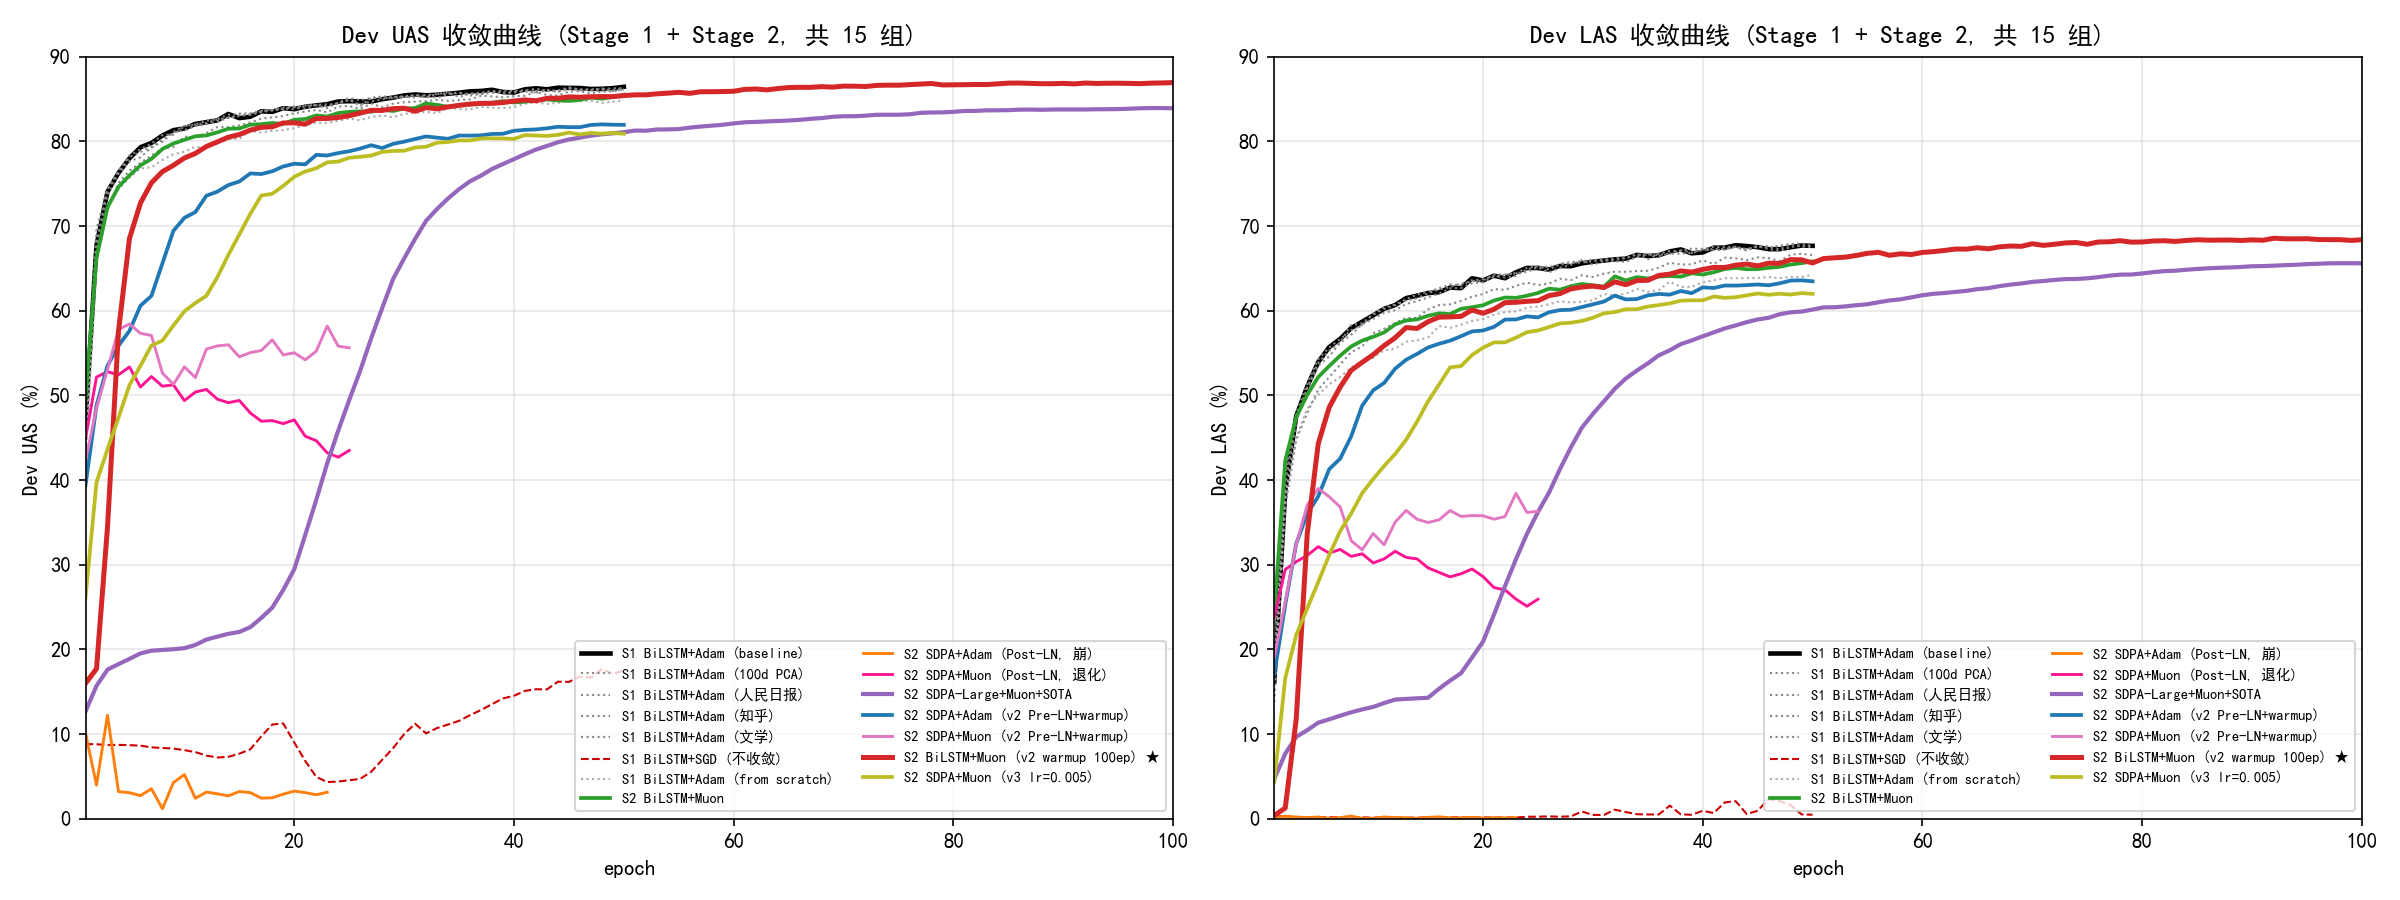
\includegraphics[width=0.98\linewidth]{figures/dev_uas_compare.png}
  \caption{Dev UAS and Dev LAS over training epochs for all fifteen configurations. The four BiLSTM curves cluster near the top ($85$--$87$ UAS), the SDPA-Large curve climbs slowly to $83.9$, the recovered SDPA-9M pre-norm curves saturate near $81$--$82$, and the two post-norm SDPA-9M curves (orange and pink) either collapse to random ($12$) or peak briefly at $53$ before retreating. Key take-away: the encoder family separates the curves more cleanly than the optimizer does, and the post-norm-no-warmup failure mode is visually unmistakable.}
  \label{fig:dev-uas}
\end{figure}

\paragraph{Post-norm SDPA-9M without warmup collapses.} Adam gives $12.20$ UAS; training UAS stays in $1$--$3\%$ throughout, confirming the model never learns. This is the textbook post-norm-without-warmup failure mode \citep{xiong2020lnorder}. Muon on the same encoder peaks at $53.35$ UAS before retreating to $43$, a partial recovery we attribute to the spectral-norm-one cap on the orthogonalized update (Section~\ref{sec:theory}).

\paragraph{Pre-norm + warmup recovers SDPA-9M.} Switching to pre-norm and adding a 500-step linear warmup yields $82.00$ UAS with Adam; for Muon we additionally reduce $\eta$ from $0.02$ to $0.005$ and obtain $81.03$ UAS. The $0.02$ Muon configuration on this same encoder early-stops at $58.42$ UAS, an effective-step-size mismatch we discuss in Section~\ref{sec:exp-encoder-discussion}.

\paragraph{SDPA-Large reaches $83.92$ UAS.} The 76M-parameter Transformer with pre-norm, RoPE, SwiGLU, LayerScale, EMA and warmup--cosine reaches its peak at epoch 99. The dev UAS curve has a slow warmup phase (first 23 epochs to $29$ UAS), a rapid main phase (epochs 23--50, climbing to $81$), and a long flat tail (epochs 50--100 adding only $2.9$ UAS). The marginal accuracy of the tail is roughly one-tenth of the marginal accuracy of the main phase, a pattern consistent with the model having absorbed the available signal.

\paragraph{BiLSTM dominates on this data scale.} The best BiLSTM ($86.93$) is $3.01$ UAS above SDPA-Large ($83.92$) despite using a sixth of the parameters. We attribute the gap to the data scale (8.3K training sentences) rather than to the encoder design itself.

\subsection{D$'$. Discussion: encoder--optimizer interaction}
\label{sec:exp-encoder-discussion}

Table~\ref{tab:encoder-optim-cross} cross-tabulates optimizer by encoder.

\begin{table}[t]
\caption{Optimizer-by-encoder dev UAS on the mixed-large 300d configuration. ``\texttt{--}'' marks combinations not run. Key take-away: Muon dominates Adam by a factor of four on the unstable post-norm SDPA, and matches Adam on the stable pre-norm SDPA, consistent with an implicit gradient-clipping interpretation of Newton--Schulz orthogonalization.}
\label{tab:encoder-optim-cross}
\centering
\small
\begin{tabular}{lrrrr}
\toprule
Optimizer & BiLSTM & SDPA-9M post-norm & SDPA-9M pre-norm & SDPA-Large \\
\midrule
Adam   & 86.43 & 12.20 & 82.00 & --     \\
Muon   & 86.93 & 53.35 & 81.03 & 83.92  \\
SGD    & 17.66 & --    & --    & --     \\
\bottomrule
\end{tabular}
\end{table}

Two observations stand out:
\begin{itemize}[leftmargin=*, itemsep=2pt]
  \item Muon's advantage over Adam is largest where training is unstable (post-norm: $53.35$ vs $12.20$, $4.4\times$) and vanishes where training is stable (pre-norm: $81.03$ vs $82.00$). This is consistent with the spectral-norm-one bound on the Muon update derived in Section~\ref{sec:theory}, which acts as an implicit gradient clipper when the raw gradient would otherwise diverge.
  \item The Muon effective step size is approximately $\eta$ (rather than $\eta/\sqrt{\hat{v}}$ as in Adam). For SDPA-9M, $\eta{=}0.02$ is too large and the model early-stops at $58.42$; reducing to $\eta{=}0.005$ recovers $81.03$. For BiLSTM, $\eta{=}0.02$ is appropriate. The right Muon learning rate scales with the model size.
\end{itemize}

\subsection{E. SDPA-Large scale-up}
\label{sec:exp-sota}

The SDPA-Large configuration combines all modern training tricks we tested (pre-norm, RoPE, SwiGLU, LayerScale, EMA, 1500-step warmup, cosine decay to $1\%$ of peak) on a 76M-parameter encoder. The peak dev UAS is $83.92$, which is $2.51$ below the BiLSTM Muon baseline. The marginal accuracy in the last 50 epochs is roughly $0.05$ UAS per epoch, suggesting the model has saturated on the available training signal. Closing the remaining gap likely requires either an order-of-magnitude increase in labeled data or initialization from a large-scale pretrained backbone such as BERT-base-Chinese; both lie outside the scope of this ablation.

\subsection{Result conclusion}
\label{sec:exp-result-conclusion}

The main empirical conclusion is not that Transformers are weak, but that the inductive bias/data-scale match dominates raw capacity in this assignment setting. The BiLSTM encoder encodes locality, order and short dependency chains directly, so 8.3K labeled sentences are enough to tune the biaffine head reliably. The SDPA encoders have a more flexible global interaction pattern, but that flexibility has to be learned from the same small supervised signal; without pre-norm and warmup it collapses, and even with a 76M-parameter modern stack it remains below the recurrent baseline.

The optimizer story is similarly conditional. Adam is the safest short-run default, SGD is a useful negative control rather than a competitive parser optimizer, and Muon becomes attractive only when the schedule gives its orthogonalized updates enough time to refine the solution. For this project, the strongest practical recipe is therefore simple: keep the original BiLSTM--biaffine architecture, use pretrained word vectors, and spend the engineering budget on a stable Muon schedule and careful logging rather than on a larger Transformer trained from scratch.
